\documentclass[11pt]{article}
\usepackage[margin=1in]{geometry}
\usepackage{graphicx}
\usepackage{amsmath}
\usepackage{booktabs}
\usepackage{url}
\usepackage[colorlinks=true,linkcolor=blue,citecolor=blue,urlcolor=blue]{hyperref}
\usepackage{listings}
\lstset{basicstyle=\small\ttfamily, columns=fullflexible, breaklines=true}

\title{Surface Mesh Analysis Pipeline for\\Al(Ga) Grain Face Characterization\\[6pt]
       {\large Addendum: May 17, 2026 Samples}}
\author{Mika Nystr\"om \and Claude (Anthropic)}
\date{May 17, 2026}

\begin{document}
\maketitle

This addendum presents curvature maps for five new grain face
samples received May~17, 2026.  The analysis uses the same pipeline
described in the main report; only the new data and its
particularities are discussed here.

Source code:
\begin{itemize}
\item Repository: \url{https://github.com/mikanystrom/intel-async} (branch \texttt{al-ga-surface-analysis})
\item Pipeline: \url{https://github.com/mikanystrom/intel-async/tree/al-ga-surface-analysis/async-toolkit/m3utils/m3utils/Al_Ga}
\end{itemize}

%% -------------------------------------------------------------------
\section{Data}

The new samples consist of five grain face meshes exported from
CloudCompare~v2.14 in \textbf{ASCII PLY} format (the earlier
samples used binary little-endian PLY).  ASCII PLY support was
added to the \texttt{plylib} reader for this dataset.

Each mesh has nine float properties per vertex: position
$(x, y, z)$, normal $(n_x, n_y, n_z)$, and original coordinates.

\begin{center}
\begin{tabular}{lrrl}
\toprule
\textbf{File} & \textbf{Vertices} & \textbf{Faces} & \textbf{Normal} \\
\midrule
Face\_1.ply & 82,409 & 164,671 & $(0.12, -0.31, 0.94)$ \\
Face\_2.ply & 99,241 & 198,331 & $(-0.17, 0.23, 0.96)$ \\
Face\_3.ply & 169,341 & 338,426 & $(-0.12, -0.50, 0.86)$ \\
Face\_4.ply & 65,329 & 130,534 & $(-0.36, -0.49, 0.80)$ \\
Face\_9.ply & 82,441 & 164,763 & $(0.05, -0.44, 0.90)$ \\
\bottomrule
\end{tabular}
\end{center}

All five faces are top-facing ($z$-component $\geq 0.80$).

\subsection{Coordinate units}

The new data uses a different coordinate system from the earlier
samples.  Empirically, a scale factor of $100$ converts the file
coordinates to micrometers, yielding face extents of $1$--$3$\,mm
consistent with the earlier dataset.  The \texttt{plydemo} tool
accepts a \texttt{-scale} parameter for this purpose:

\begin{lstlisting}
plydemo -contour outdir -scale 100 data_2026_05_17/Face_1.ply
\end{lstlisting}

%% -------------------------------------------------------------------
\section{Curvature Atlas}

The following pages present cotangent-Laplacian mean curvature maps
for all five faces.  All plots share a common color scale of
$[-3, +3]$\,mm$^{-1}$, with gray at zero (flat), red for convex,
and blue for concave regions.  Coordinates are in micrometers.
Axis scales are identical in $x$ and $y$.

\clearpage
\subsection*{Sample data\_2026\_05\_17}
\begin{center}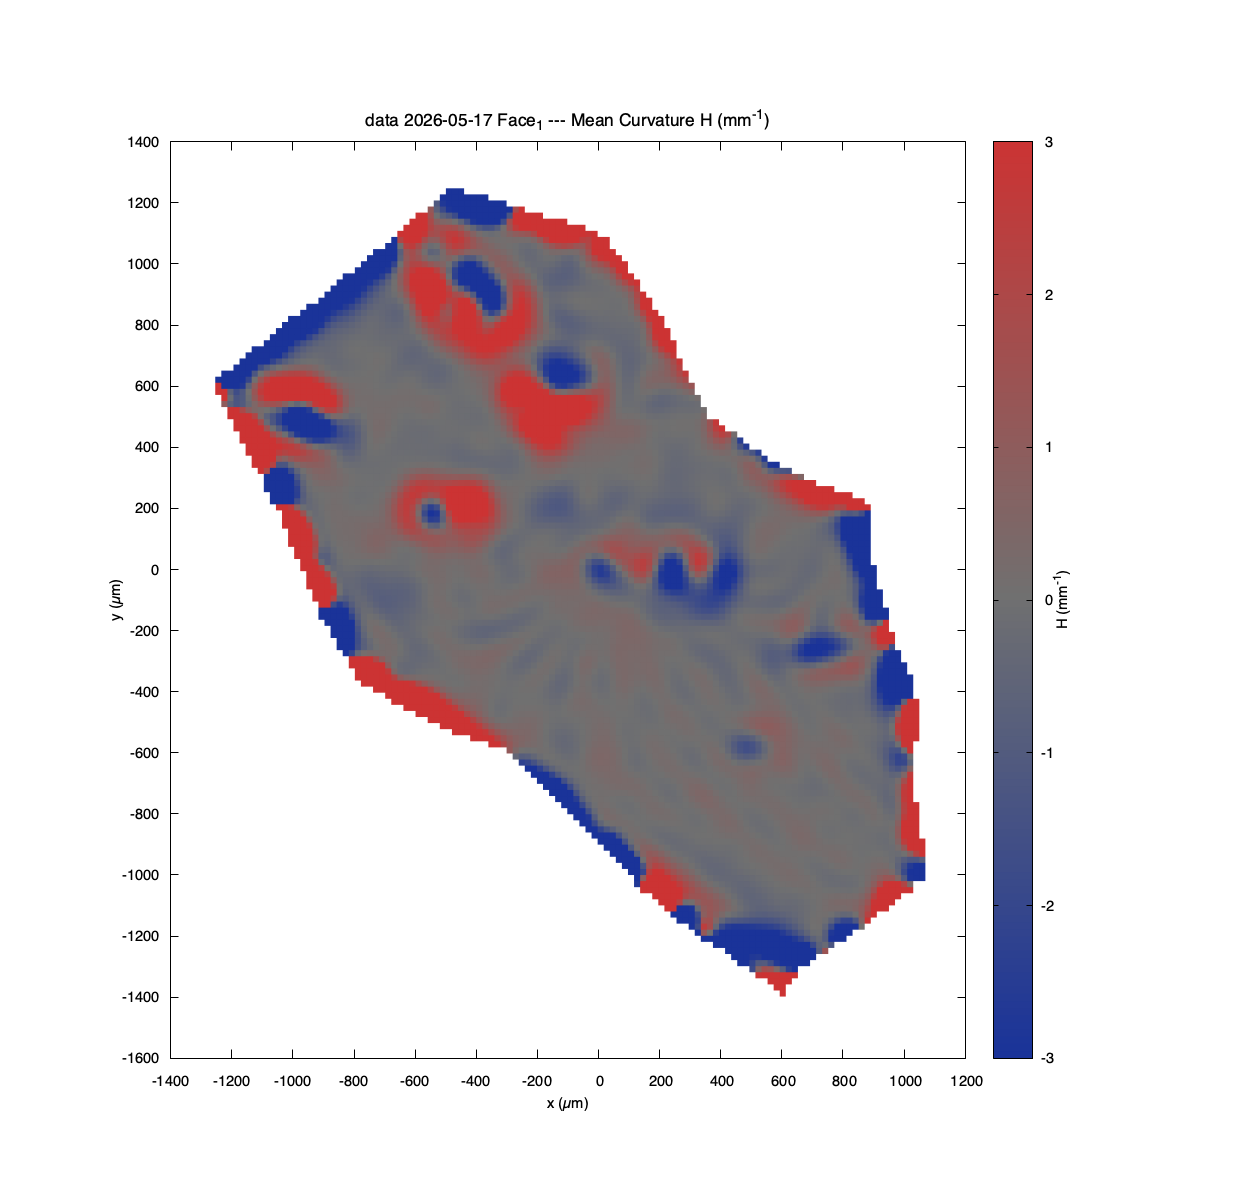
\includegraphics[width=0.75\textwidth]{figures/new-Face_1.png}\end{center}
\begin{center}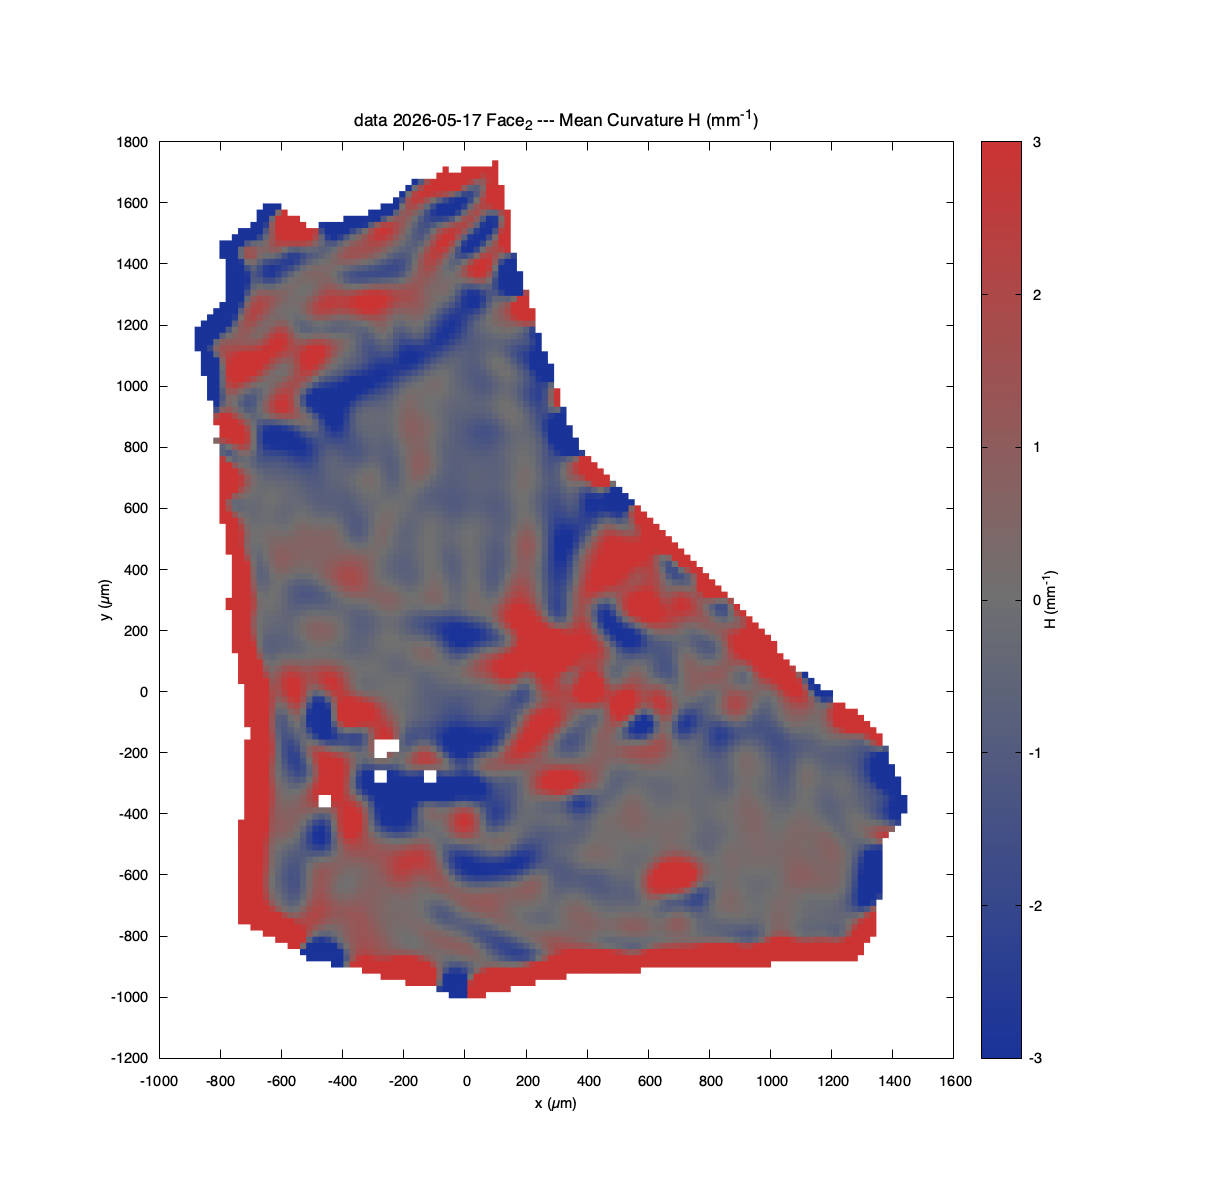
\includegraphics[width=0.75\textwidth]{figures/new-Face_2.png}\end{center}
\begin{center}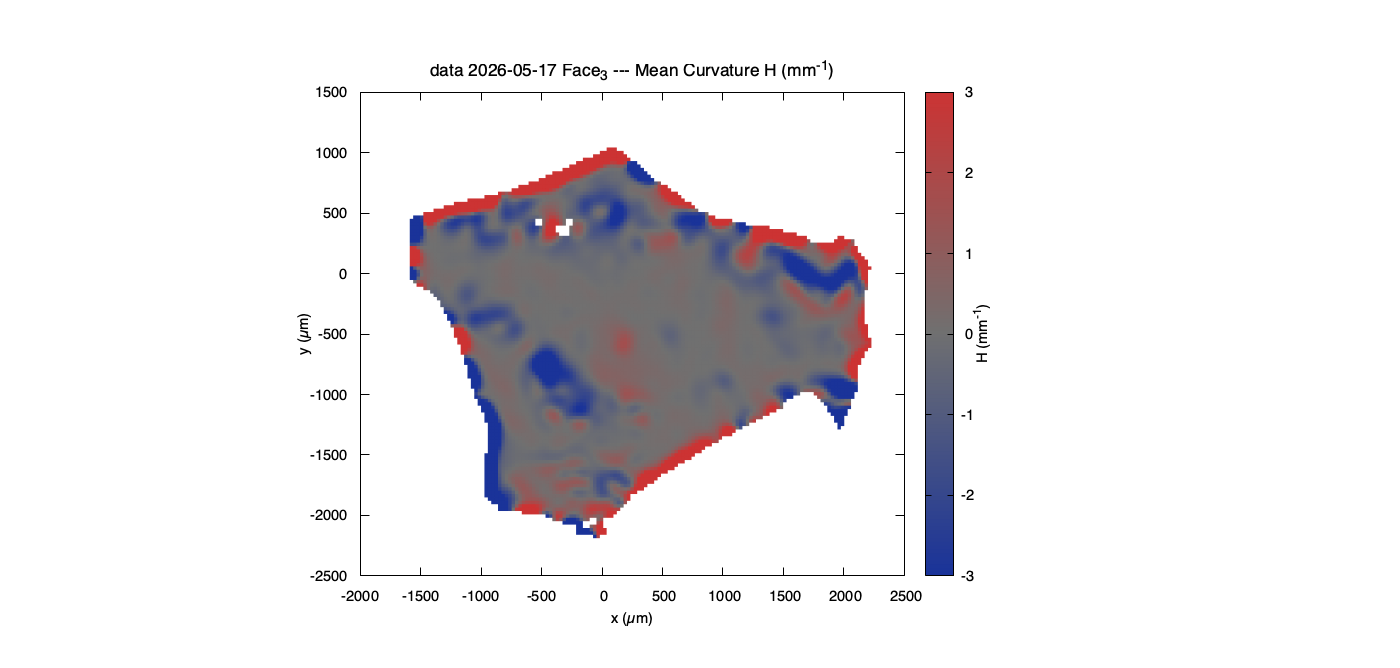
\includegraphics[width=0.75\textwidth]{figures/new-Face_3.png}\end{center}
\begin{center}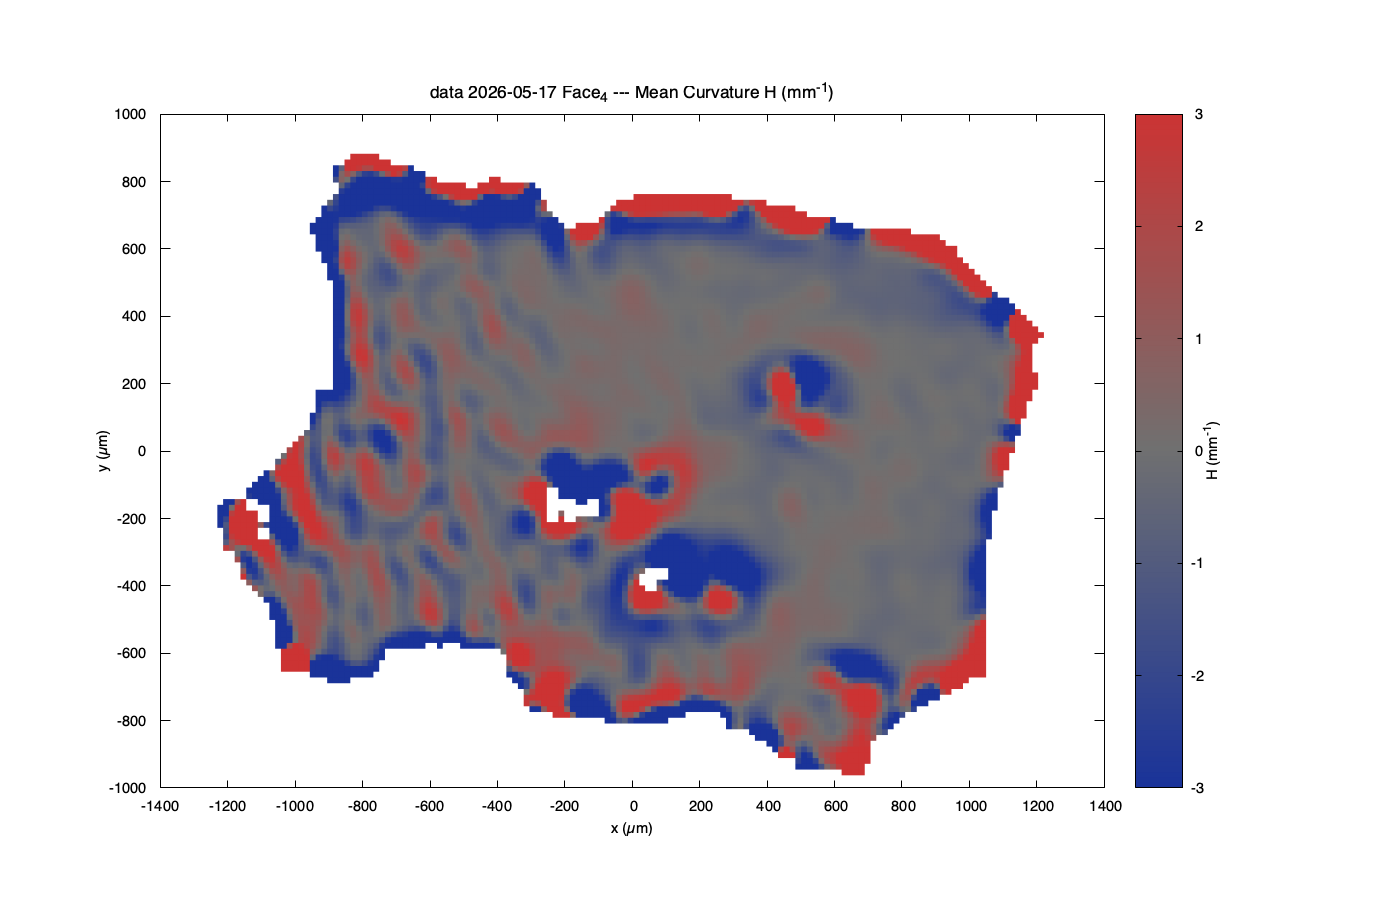
\includegraphics[width=0.75\textwidth]{figures/new-Face_4.png}\end{center}
\begin{center}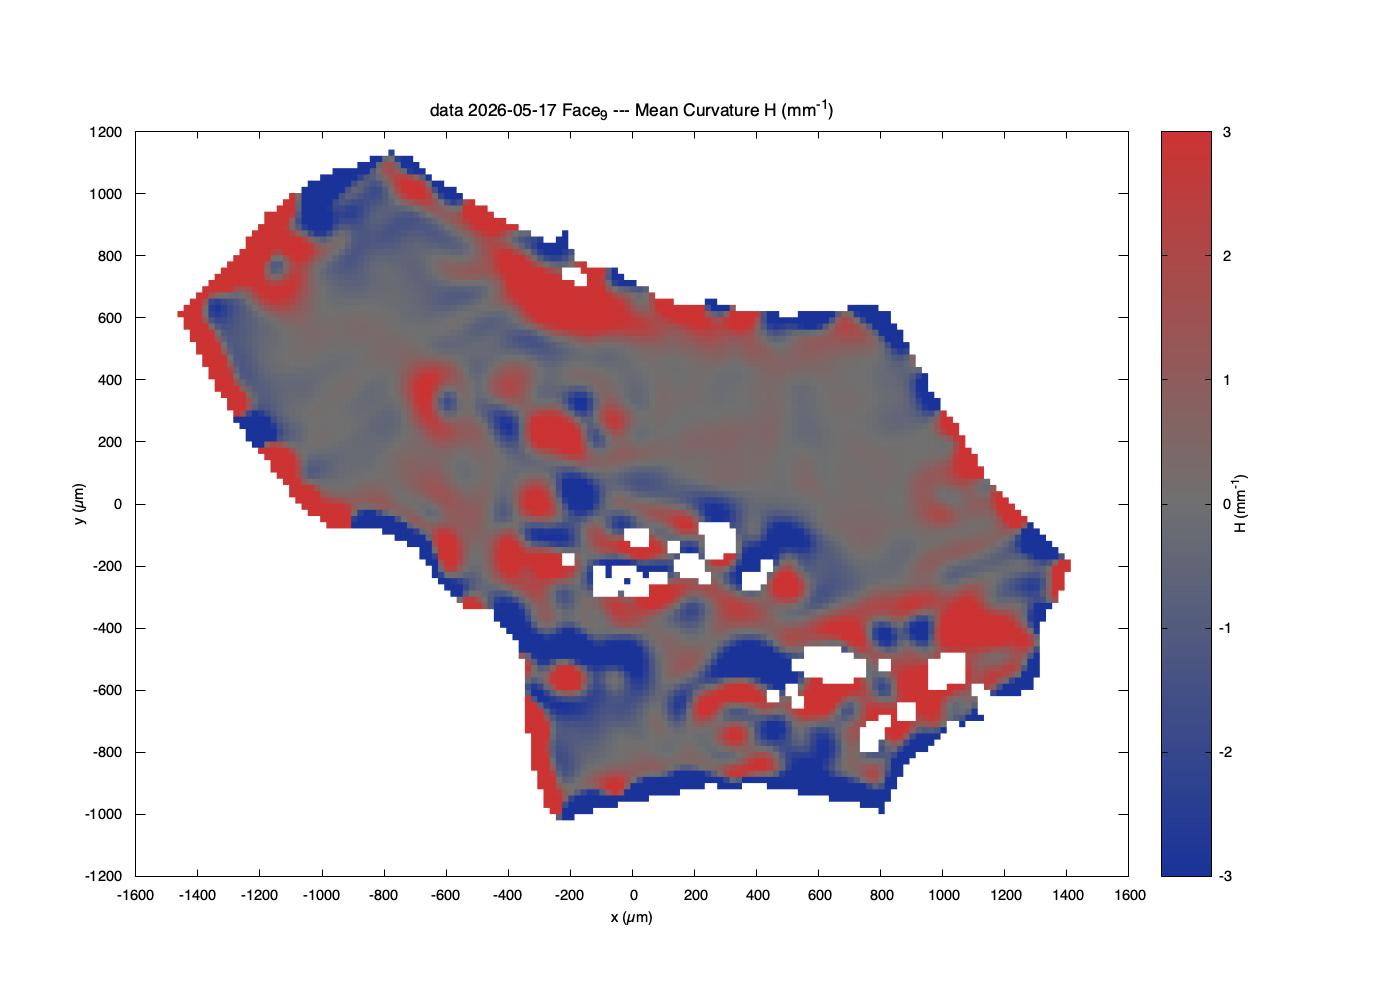
\includegraphics[width=0.75\textwidth]{figures/new-Face_9.png}\end{center}

\end{document}
